\PassOptionsToPackage{unicode=true}{hyperref} % options for packages loaded elsewhere
\PassOptionsToPackage{hyphens}{url}
%
\documentclass[english,man,man,floatsintext]{apa6}
\usepackage{lmodern}
\usepackage{amssymb,amsmath}
\usepackage{ifxetex,ifluatex}
\usepackage{fixltx2e} % provides \textsubscript
\ifnum 0\ifxetex 1\fi\ifluatex 1\fi=0 % if pdftex
  \usepackage[T1]{fontenc}
  \usepackage[utf8]{inputenc}
  \usepackage{textcomp} % provides euro and other symbols
\else % if luatex or xelatex
  \usepackage{unicode-math}
  \defaultfontfeatures{Ligatures=TeX,Scale=MatchLowercase}
\fi
% use upquote if available, for straight quotes in verbatim environments
\IfFileExists{upquote.sty}{\usepackage{upquote}}{}
% use microtype if available
\IfFileExists{microtype.sty}{%
\usepackage[]{microtype}
\UseMicrotypeSet[protrusion]{basicmath} % disable protrusion for tt fonts
}{}
\IfFileExists{parskip.sty}{%
\usepackage{parskip}
}{% else
\setlength{\parindent}{0pt}
\setlength{\parskip}{6pt plus 2pt minus 1pt}
}
\usepackage{hyperref}
\hypersetup{
            pdftitle={Experience with research paradigms relates to infants' direction of preference.},
            pdfkeywords={preferential looking, familiarity preference, novelty preference, head-turn preference procedure, linear mixed-effects model},
            pdfborder={0 0 0},
            breaklinks=true}
\urlstyle{same}  % don't use monospace font for urls
\usepackage{longtable,booktabs}
% Fix footnotes in tables (requires footnote package)
\IfFileExists{footnote.sty}{\usepackage{footnote}\makesavenoteenv{longtable}}{}
\usepackage{graphicx,grffile}
\makeatletter
\def\maxwidth{\ifdim\Gin@nat@width>\linewidth\linewidth\else\Gin@nat@width\fi}
\def\maxheight{\ifdim\Gin@nat@height>\textheight\textheight\else\Gin@nat@height\fi}
\makeatother
% Scale images if necessary, so that they will not overflow the page
% margins by default, and it is still possible to overwrite the defaults
% using explicit options in \includegraphics[width, height, ...]{}
\setkeys{Gin}{width=\maxwidth,height=\maxheight,keepaspectratio}
\setlength{\emergencystretch}{3em}  % prevent overfull lines
\providecommand{\tightlist}{%
  \setlength{\itemsep}{0pt}\setlength{\parskip}{0pt}}
\setcounter{secnumdepth}{0}

% set default figure placement to htbp
\makeatletter
\def\fps@figure{htbp}
\makeatother

% Manuscript styling
\usepackage{upgreek}
\captionsetup{font=singlespacing,justification=justified}

% Table formatting
\usepackage{longtable}
\usepackage{lscape}
% \usepackage[counterclockwise]{rotating}   % Landscape page setup for large tables
\usepackage{multirow}		% Table styling
\usepackage{tabularx}		% Control Column width
\usepackage[flushleft]{threeparttable}	% Allows for three part tables with a specified notes section
\usepackage{threeparttablex}            % Lets threeparttable work with longtable

% Create new environments so endfloat can handle them
% \newenvironment{ltable}
%   {\begin{landscape}\begin{center}\begin{threeparttable}}
%   {\end{threeparttable}\end{center}\end{landscape}}
\newenvironment{lltable}{\begin{landscape}\begin{center}\begin{ThreePartTable}}{\end{ThreePartTable}\end{center}\end{landscape}}

% Enables adjusting longtable caption width to table width
% Solution found at http://golatex.de/longtable-mit-caption-so-breit-wie-die-tabelle-t15767.html
\makeatletter
\newcommand\LastLTentrywidth{1em}
\newlength\longtablewidth
\setlength{\longtablewidth}{1in}
\newcommand{\getlongtablewidth}{\begingroup \ifcsname LT@\roman{LT@tables}\endcsname \global\longtablewidth=0pt \renewcommand{\LT@entry}[2]{\global\advance\longtablewidth by ##2\relax\gdef\LastLTentrywidth{##2}}\@nameuse{LT@\roman{LT@tables}} \fi \endgroup}

% \setlength{\parindent}{0.5in}
% \setlength{\parskip}{0pt plus 0pt minus 0pt}

% \usepackage{etoolbox}
\makeatletter
\patchcmd{\HyOrg@maketitle}
  {\section{\normalfont\normalsize\abstractname}}
  {\section*{\normalfont\normalsize\abstractname}}
  {}{\typeout{Failed to patch abstract.}}
\makeatother
\shorttitle{Direction of preference in infancy}
\author{Chiara Santolin\textsuperscript{1}, Gonzalo Garcia-Castro\textsuperscript{1}, Martin Zettersten\textsuperscript{2}, Nuria Sebastian-Galles\textsuperscript{1}, \& Jenny Saffran\textsuperscript{2}}
\affiliation{
\vspace{0.5cm}
\textsuperscript{1} Center for Brain and Cognition, Universitat Pompeu Fabra\\\textsuperscript{2} Waisman Center \& Department of Psychology, University of Wisconsin-Madison}
\authornote{

Correspondence concerning this article should be addressed to Chiara Santolin, Edifici Merce Rodereda, Calle Ramón Trias Fargas, 25, 08018 Barcelona. E-mail: chiara.santolin@upf.edu}
\note{Preprint submitted to peer-review on February, 17th, 2020}
\keywords{preferential looking, familiarity preference, novelty preference, head-turn preference procedure, linear mixed-effects model\newline\indent Word count: 2939}
\usepackage{lineno}

\linenumbers
\usepackage{csquotes}
\ifnum 0\ifxetex 1\fi\ifluatex 1\fi=0 % if pdftex
  \usepackage[shorthands=off,main=english]{babel}
\else
  % load polyglossia as late as possible as it *could* call bidi if RTL lang (e.g. Hebrew or Arabic)
  \usepackage{polyglossia}
  \setmainlanguage[]{english}
\fi

\title{Experience with research paradigms relates to infants' direction of preference.}

\date{}

\abstract{
Interpreting and predicting direction of preference in infant behavioral research has been a thorny issue for decades. Several factors have been proposed to account for familiarity and novelty preferences in habituation and familiarization studies, including infant age, length of exposure and task complexity. The current study explores an additional dimension that may affect direction of preference: amount of experience with the experimental task. To test this hypothesis, we re-analyzed the data from 4 experiments on artificial grammar learning in 12-month-old infants run using the Head- turn Preference Procedure (HPP). The participants in these studies varied substantially in their number of laboratory visits. Linear mixed-effects results show that the number of HPP studies in which infants had previously participated is related to infants' direction of preference: infants who had no (or limited) experience with the HPP setting were more likely to show familiarity preferences than infants who had amassed more experience with this task in prior study visits. Interestingly, the effect is driven by a significant decrease in looking time for familiar trials. These results have important implications for the interpretation of experimental results: infants' experience with a given paradigm or, more broadly, with the lab environment, may affect their patterns of preferences.
}

\begin{document}
\maketitle

\hypertarget{introduction}{%
\section{Introduction}\label{introduction}}

In infancy research, the importance of changes in preferential looking has been recognized since at least the 1960s, when Fantz (1964) showed that young infants preferentially attend to novel visual stimuli. Subsequent studies extended this evidence to other domains, including acoustic perception and cognition, revealing differences in direction of preference. Theories intended to account for such differences suggest that novelty preferences arise when infants have completed the processing of a (familiar) stimulus (see Houston‐Price \& Nakai, 2004; and Aslin, 2007 for reviews).

Rather than representing a binary distinction, direction of preference can be construed as a continuum from more familiar to more novel (e.g., Thiessen, Hill, \& Saffran, 2005). Hunter and Ames (1988) provide the most comprehensive model of preferential looking with three central factors hypothesized to affect the strength and direction of preference: age, familiarization duration and task complexity. In a given task, younger infants tend to prefer the familiar stimulus whereas older infants are more likely to prefer the novel one (e.g., Colombo \& Bundy, 1983; though see Bergmann \& Cristia, 2016, for a meta-analysis suggesting that age does not predict shifts in preference). A shorter exposure to familiar stimulus prior to testing also leads infants to subsequently prefer the familiar object (for reviews, see also Rose, Feldman, \& Jankowski, 2004). Task complexity refers to the stage of stimulus processing. For example, in a visual recognition task, 4-month-old infants revealed a systematic preference for the familiar object prior to showing a strong preference for the novel object (Roder, Bushneil, \& Sasseville, 2000). Task complexity can also refer to the complexity of stimuli. For example, sequential stimuli put greater strain on memory resources than stimuli in which all components are simultaneously available (e.g., Ferguson, Franconeri, \& Waxman, 2018). A related dimension is the similarity across stimuli used at familiarization and test: when there is a close perceptual match such as same colors or sounds during training and test, infants are more likely to show a novelty preference (e.g., Hunter \& Ames, 1988; Thiessen \& Saffran, 2003).

The combination of these factors informs predictions concerning direction of preference in systematic ways. For example, Thiessen et al. (2005) manipulated length of exposure and observed a flip from familiarity to novelty preference after doubling the amount of familiarization received by the infants. Similarly, Ferguson et al. (2018) manipulated sequential vs.~spatial presentation of visual patterns, and observed stronger novelty effects with (a) increasing age and (b) spatial presentation. That said, it is also frequently the case that the observed direction of preference does not conform with expectations based on the dimensions noted above; the infancy literature is rife with examples of counterintuitive patterns of preference (e.g., Fiser and Aslin (2001); Thiessen (2012) for post-habituation familiarity preference; Bosch and Sebastián‐Gallés (2001); Sebastián-Gallés and Bosch (2009); Dawson and Gerken (2009) for novelty preference in 4-month-olds; Jusczyk and Aslin (1995) for familiarity preference in 7-months-olds; Johnson et al. (2009) for both novelty and familiarity preference in 11-months-olds).

One factor that is frequently overlooked in considerations of infant data is that infants do not arrive at the lab as naïve participants. Like adults, they bring significant prior experience that may influence their performance in lab tasks. In many instances, researchers attempt to override or sidestep those experiences by using novel stimuli (e.g., unfamiliar languages, shapes or sounds), or by integrating those experiences into their experimental designs (e.g., monolingual vs.~bilingual infants). But there may also be forms of experience that go unidentified by researchers. One such factor is that many infants participate in more than one experiment over the course of weeks or months. Testing the same participants in multiple (putatively unrelated) experiments is a common practice in infant research, reflecting the challenges of advancing a field of investigation that is based on a limited and hard-to-recruit population. Researchers are typically very careful to avoid stimulus contagion across unrelated studies, but it is possible that prior lab experience impacts infants' performance.

The purpose of this article is to explore the effect of experience with experimental paradigms on direction of preference in learning tasks. This idea emerged from a puzzling pattern of results in a replication of a published study focused on non-linguistic artificial grammar learning in 12-month-olds (Santolin \& Saffran, 2019). We observed a flip in preference from novelty to familiarity between the original study and its replication (Santolin et al., 2019), despite the use of identical stimuli and procedures. While there were some differences between the studies (most notably, in the location in which the studies were run), one main factor stood out to us: many of the infants in the study that elicited a novelty preference had participated in prior studies with Head-turn Preference Procedure (HPP), whereas most of the infants in the study that elicited a familiarity preference were first-time HPP participants. We reasoned that the more familiarity infants had with the lab apparatus and task demands, the more likely they would be to learn rapidly, leading to a novelty preference. To explore this question, we combined the data from these two experiments with the data from two other published artificial grammar learning tasks with similar designs that included 12-month-olds with a range in number of lab visits (Saffran et al., 2008, Exp. 1 Language P; and Saffran \& Wilson, 2003, Exp. 2). Our hypothesis was that the amount of infants' prior experience with HPP would affect direction of preference.

\hypertarget{methods}{%
\section{Methods}\label{methods}}

A brief description of the four experiments included in this analysis, and our rationale for selecting them, is provided in the Appendix A, S1 (see Figure 1) for a summary of the results). A fully reproducible repository hosting data and analyses is available at \url{https://osf.io/g95ub/}.

\begin{figure}
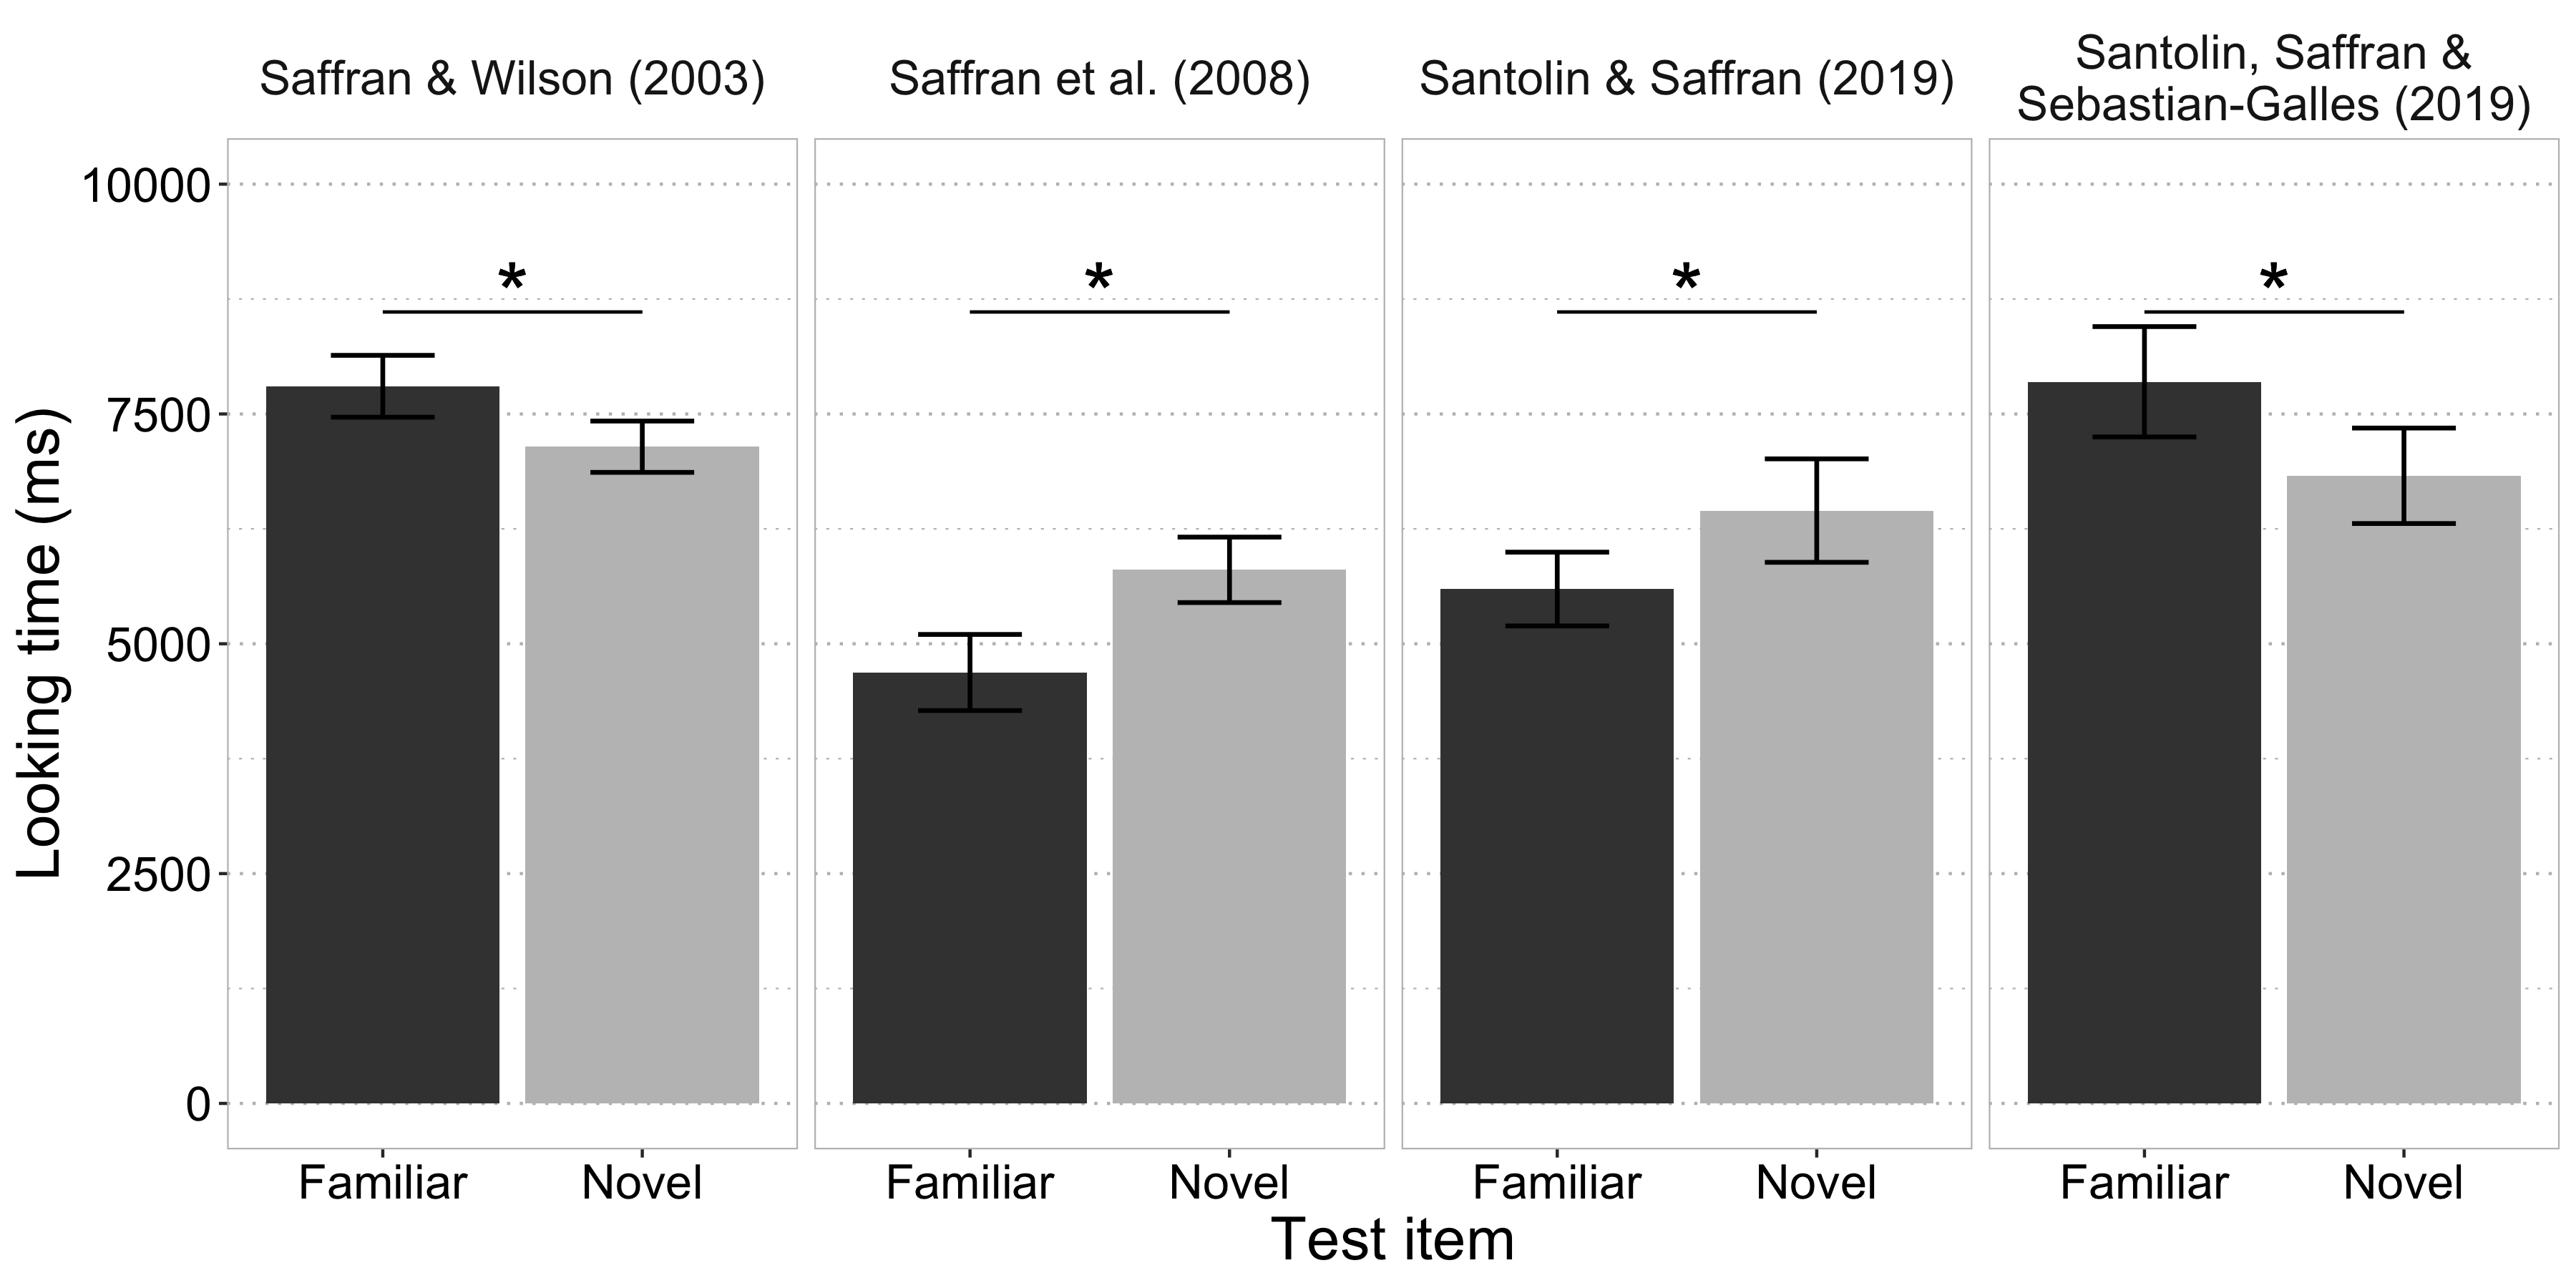
\includegraphics[width=\textwidth]{/Users/GonzaloGGC/projects/Flip/Figures/01_lookingtimes-study} \caption{Looking time for familiar and novel test stimuli of the original studies. Stimuli vary based on the experiment. Error bars indicate the standard error of the mean.}\label{fig:fig1}
\end{figure}

We modeled results of all infants (\emph{N}=102) who participated in the four studies. Number of HPP visits varied from one to six total visits (including the current visit). We fit a linear mixed-effect model including \emph{Looking time} as the response variable, and \emph{Test item} (Familiar vs.~Novel), \emph{HPP} (number of experiments completed by infants) and their interaction as fixed effects. We especified a nested random effects structure, with participants nested wihtin studies (each participant was inluded in only one study). We included by-participant and by-study random intercepts (4 levels: Santolin \& Saffran, 2019; Santolin, Saffran, \& Sebastian-Galles, 2019; Saffran et al., 2008; Saffran \& Wilson, 2003). The \emph{HPP} predictor was coded as a continuous variable indicating the overall number of experiments with the Head-turn Preference Procedure the infants participated in. \emph{Test Item }was centered on familiar test items (Familiar = 0; Novel = 1). Since the experiments differ at distinct levels (e.g., different stimuli, lab location), the model accounted for cross-participant and cross-study differences in looking time. Degrees of freedom were approximated using the Kenward-Roger approach (Judd, Westfall, \& Kenny, 2012), which can result in non-integer values. Further modeling details are provided in Appendix A, S3.

We predicted a \emph{Test item} (familiar vs.~novel) by number of \emph{HPP} interaction, indicating that the duration of infants' looking towards familiar versus novel items would depend on infants' HPP experience. An interaction could result from at least three different patterns of results: an increase in looking time for novel items, a decrease in looking time for familiar items, or both, as a result of additional experience in HPP studies.

\hypertarget{results}{%
\section{Results}\label{results}}

We found a statistically significant interaction (\emph{F}(1,100.00) = 11.99, \emph{p} = .001) suggesting that the effect of Test Items on looking time differences was affected by the number of HPP experiments infants had participated in (Table 1, Figure 2). In line with our predictions, the size of the difference between looking times on familiar and novel test items changed as a function of number of HPP visits.

We also found a significant main effect of the HPP predictor (\emph{F}(1,133.10) = 4.80, \emph{p} = .030) indicating that the Test Item by HPP interaction is mainly driven by a significant decrease in looking time to familiar items as the number of HPP visits increases. There was no evidence that a greater number of HPP visits was accompanied by longer looking to the novel item (\emph{F}(1,133.10) = 0.27, \emph{p} = .606).

Results also hold when reducing the data to infants with less than six HPP indicating that the interaction effect was not driven exclusively by participants with an unusually high number of visits {[}HPP 1-5: \emph{F}(1,99.00) = 10.29, \emph{p} = .002; HPP 1-4: \emph{F}(1,98.00) = 10.43, \emph{p} = .002; HPP 1-3: \emph{F}(1,92.00) = 4.56, \emph{p} = .035{]}. Notably, the interaction is significant even when sub-setting the data to the infants who participated in two HPP experiments only (HPP 1-2: \emph{F}(1,78.00) = 4.05, \emph{p} = .048).

\begin{longtable}[]{@{}lcccccc@{}}
\caption{\label{tab:tab1}Summary of the results of the linear mixed-effects model.}\tabularnewline
\toprule
& \textbf{Coefficient} & \textbf{\emph{SEM}} & \textbf{95\% CI} & \textbf{\emph{F}} & \textbf{Den. \emph{df}} & \textbf{\emph{p}}\tabularnewline
\midrule
\endfirsthead
\toprule
& \textbf{Coefficient} & \textbf{\emph{SEM}} & \textbf{95\% CI} & \textbf{\emph{F}} & \textbf{Den. \emph{df}} & \textbf{\emph{p}}\tabularnewline
\midrule
\endhead
\emph{Intercept} & 7,679.1 & 673.1 & {[}6390.1, 9294.1{]} & 124.7 & 9.1 & \textless{} .001\tabularnewline
\emph{Test Item} & -1,398.8 & 411.3 & {[}-2204.8, -589.1{]} & 11.6 & 100.0 & .001\tabularnewline
\emph{HPP} & -539.7 & 238.7 & {[}-999.9, -74.8{]} & 4.8 & 133.1 & .030\tabularnewline
\emph{Test Item \(\times\) HPP} & 667.1 & 192.6 & {[}247.2, 1028.5{]} & 12.0 & 100.0 & .001\tabularnewline
\bottomrule
\end{longtable}

\begin{figure}
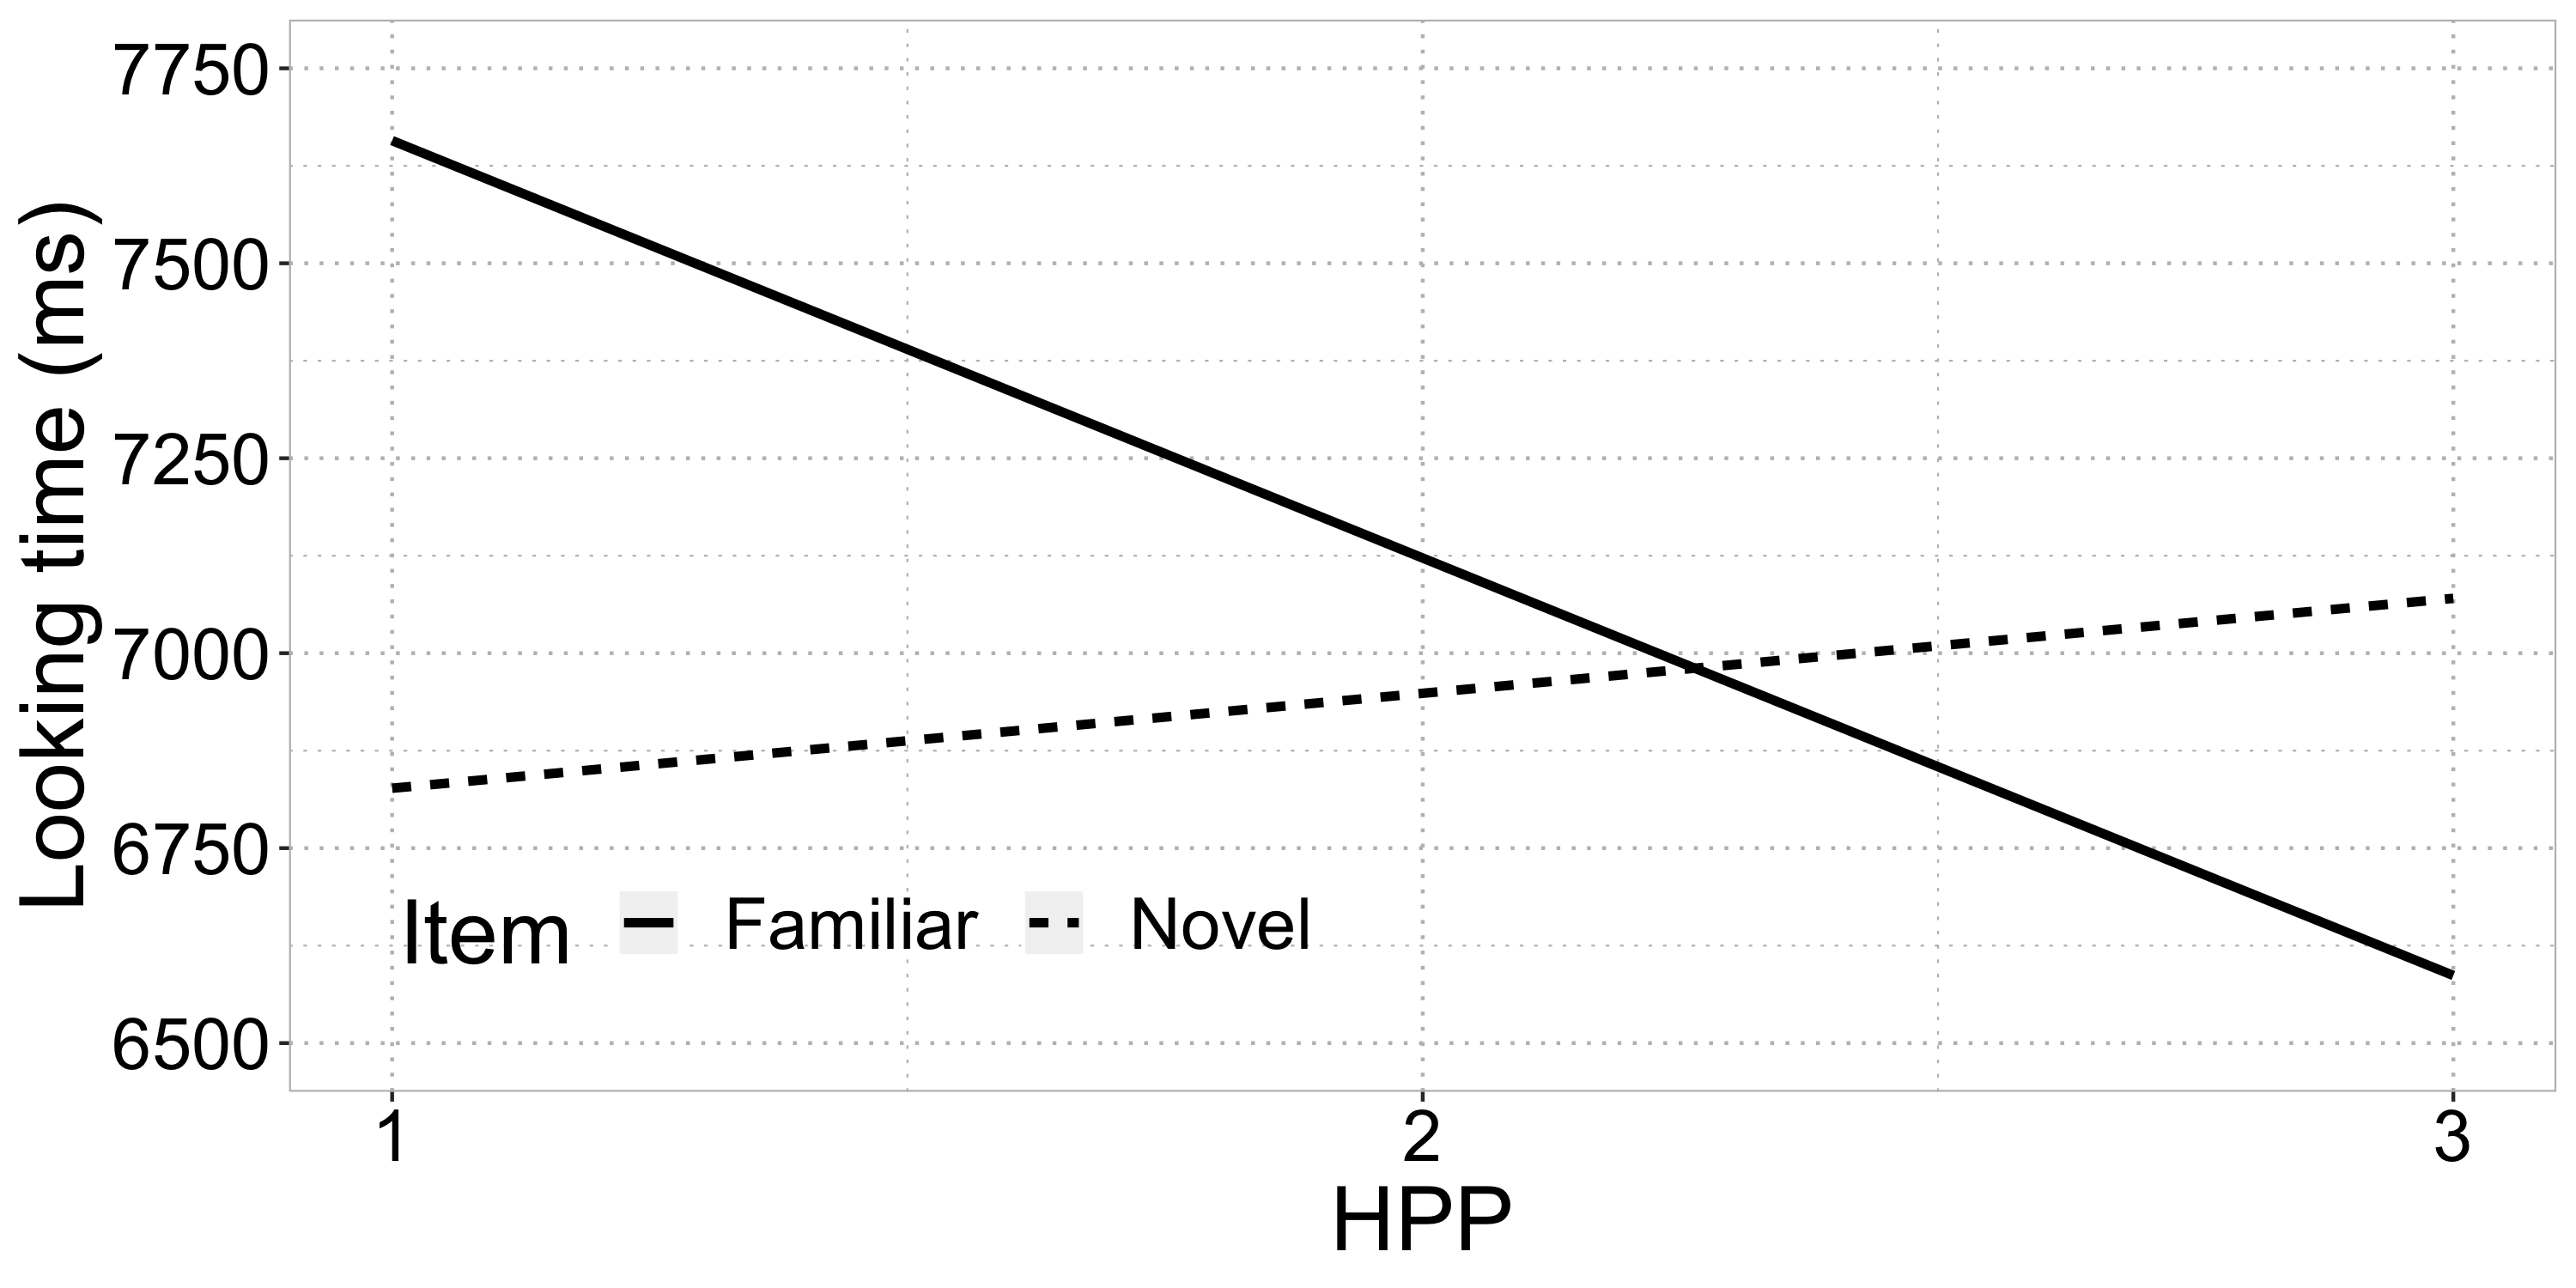
\includegraphics[width=\textwidth]{/Users/GonzaloGGC/projects/Flip/Figures/03_interaction} \caption{Panel A: graphic representation of the coefficients of the fixed effects of the model. Black dots represent the point estimate of the coefficient, black whiskers represent the standard error of the mean, and grey boxes represent the bootstrapped 95\% confidence interval around the point estimate. Panel B: predicted looking time (in ms) for familiar and novel test items plotted against number of HPP visits. Black dots and lines represent the mean predicted looking time, and grey shaded areas represent the standard error of the mean.}\label{fig:fig2}
\end{figure}

\hypertarget{discussion}{%
\section{Discussion}\label{discussion}}

Results reported in this article are consistent with our hypothesis that experience with the Head-turn Preference Procedure affects direction of preference. The model combined four experiments with 12-month-old infants performing simple artificial grammar learning tasks, and showed that infants who had \emph{not} previously experienced the HPP setting were more likely to show familiarity preferences than infants who had prior experience. One possible explanation for this finding relates to the structure of the HPP task. There are at least two types of information that must be simultaneously encoded by the infant at her first HPP experiment: 1) visual-auditory contingency (i.e., sounds appear contingently on the infant looking at the screen), and 2) the experiment stimuli (e.g., word sequences, sound streams). Therefore, infants have to engage in two concurrent learning when experiencing HPP for the first time: learning the structure of the HPP method, and solving the learning problem itself (e.g., discriminating sound strings following/breaking the grammar patterns). Such double-processing of information likely increases the task complexity, biasing results towards familiarity preferences. Infants who return to the lab for subsequent HPP experiments may be more able to focus on the learning problem, resulting in better learning as evidenced in novelty preferences.

It is important to notice that this effect may not just be limited to experiencing the HPP setting \emph{per se}, but can be caused by the entire laboratory visit. When infants visit the lab for the very first time, they face a challenging situation: a new environment with new people interacting with them, testing rooms with a peculiar design (e.g., all-black or all-white walls with big screens), and novel sounds and images. This is a great amount of novel information for a young infant to process at once. In contrast, as infants come back to the lab for subsequent studies, the location, testing room and research staff may become more familiar, reducing the information load. The present study cannot discern which type of previous experience (HPP setting or lab) is responsible for the observed results.

Our findings have important implications for the interpretation of directions of preference in future studies. Infants' prior experience with a lab or research paradigm could account for distinct, and sometimes counterintuitive, patterns of preference. A related hypothesis suggests that less-common directions of preference for studies addressing a given topic (e.g., rule learning) likely represent sign errors as opposed to true infant preferences {[}Rabagliati, Ferguson, and Lew-Williams (2019); Bergmann, Rabagliati, and Tsuji (2019); RR{]}. While this may be the case, it is also possible that discrepancies in preferential looking are related to factors like those investigate in the current study: prior experience with the testing environment. For this reason, discrepancies such as unexpected directions of preference may actually be meaningful and informative about the state of infant learners in specific studies.

These results would allow to update the model of the factors inducing different patterns of preferences in infant studies (e.g., Hunter \& Ames, 1988). Here we propose that the dimension \emph{task complexity} could be expanded beyond the specific task content (e.g., how complex are the stimuli presented) to include infants' familiarity with the task. Our findings, in fact, suggest that the learning outcome of a given task is constrained by how much task experience infants have accumulated through prior lab visits. Therefore, the amount of novel information infants have to process in parallel during a study increases the task demands, and the likelihood of showing a familiarity preference. This may well include the novelty of the experimental paradigm. It would be of great interest to expand our findings to other preferential paradigms (e.g., infant-controlled preferential looking procedures, visual-world paradigms) to advance our understanding of how such experiences modulate infants' performance at test.

\newpage

\hypertarget{references}{%
\section{References}\label{references}}

\begingroup
\setlength{\parindent}{-0.5in}
\setlength{\leftskip}{0.5in}

\hypertarget{refs}{}
\leavevmode\hypertarget{ref-aslin2007}{}%
Aslin, R. N. (2007). What's in a look? \emph{Developmental Science}, \emph{10}(1), 48--53. \url{https://doi.org/10.1111/j.1467-7687.2007.00563.x}

\leavevmode\hypertarget{ref-bergmann2016}{}%
Bergmann, C., \& Cristia, A. (2016). Development of infants' segmentation of words from native speech: A meta-analytic approach. \emph{Developmental Science}, \emph{19}(6), 901--917. \url{https://doi.org/10.1111/desc.12341}

\leavevmode\hypertarget{ref-bergmann2019}{}%
Bergmann, C., Rabagliati, H., \& Tsuji, S. (2019). What's in a looking time preference? \url{https://doi.org/10.31234/osf.io/6u453}

\leavevmode\hypertarget{ref-bosch2001}{}%
Bosch, L., \& Sebastián‐Gallés, N. (2001). Evidence of Early Language Discrimination Abilities in Infants From Bilingual Environments. \emph{Infancy}, \emph{2}(1), 29--49. \url{https://doi.org/10.1207/S15327078IN0201_3}

\leavevmode\hypertarget{ref-colombo1983}{}%
Colombo, J., \& Bundy, R. S. (1983). Infant response to auditory familiarity and novelty. \emph{Infant Behavior \& Development}, \emph{6}(3), 305--311. \url{https://doi.org/10.1016/S0163-6383(83)80039-3}

\leavevmode\hypertarget{ref-dawson2009}{}%
Dawson, C., \& Gerken, L. (2009). From Domain-Generality to Domain-Sensitivity: 4-Month-Olds Learn an Abstract Repetition Rule in Music That 7-Month-Olds Do Not. \emph{Cognition}, \emph{111}(3), 378--382. \url{https://doi.org/10.1016/j.cognition.2009.02.010}

\leavevmode\hypertarget{ref-fantz1964}{}%
Fantz, R. L. (1964). Visual Experience in Infants: Decreased Attention to Familiar Patterns Relative to Novel Ones. \emph{Science}, \emph{146}(3644), 668--670. \url{https://doi.org/10.1126/science.146.3644.668}

\leavevmode\hypertarget{ref-ferguson2018}{}%
Ferguson, B., Franconeri, S. L., \& Waxman, S. R. (2018). Very young infants learn abstract rules in the visual modality. \emph{PloS One}, \emph{13}(1), e0190185. \url{https://doi.org/10.1371/journal.pone.0190185}

\leavevmode\hypertarget{ref-fiser2001}{}%
Fiser, J., \& Aslin, R. N. (2001). Unsupervised statistical learning of higher-order spatial structures from visual scenes. \emph{Psychological Science}, \emph{12}(6), 499--504. \url{https://doi.org/10.1111/1467-9280.00392}

\leavevmode\hypertarget{ref-houston-price2004}{}%
Houston‐Price, C., \& Nakai, S. (2004). Distinguishing novelty and familiarity effects in infant preference procedures. \emph{Infant and Child Development}, \emph{13}(4), 341--348. \url{https://doi.org/10.1002/icd.364}

\leavevmode\hypertarget{ref-hunter1988}{}%
Hunter, M. A., \& Ames, E. W. (1988). A multifactor model of infant preferences for novel and familiar stimuli. In \emph{Advances in infancy research, Vol. 5.} (pp. 69--95). Westport, CT, US: Ablex Publishing.

\leavevmode\hypertarget{ref-johnson2009}{}%
Johnson, S. P., Fernandes, K. J., Frank, M. C., Kirkham, N., Marcus, G., Rabagliati, H., \& Slemmer, J. A. (2009). Abstract Rule Learning for Visual Sequences in 8- and 11-Month-Olds. \emph{Infancy : The Official Journal of the International Society on Infant Studies}, \emph{14}(1), 2--18. \url{https://doi.org/10.1080/15250000802569611}

\leavevmode\hypertarget{ref-judd2012}{}%
Judd, C. M., Westfall, J., \& Kenny, D. A. (2012). Treating stimuli as a random factor in social psychology: A new and comprehensive solution to a pervasive but largely ignored problem. \emph{Journal of Personality and Social Psychology}, \emph{103}(1), 54--69. \url{https://doi.org/10.1037/a0028347}

\leavevmode\hypertarget{ref-jusczyk1995}{}%
Jusczyk, P. W., \& Aslin, R. N. (1995). Infants' detection of the sound patterns of words in fluent speech. \emph{Cognitive Psychology}, \emph{29}(1), 1--23. \url{https://doi.org/10.1006/cogp.1995.1010}

\leavevmode\hypertarget{ref-rabagliati2019}{}%
Rabagliati, H., Ferguson, B., \& Lew-Williams, C. (2019). The profile of abstract rule learning in infancy: Meta-analytic and experimental evidence. \emph{Developmental Science}, (1), e12704. \url{https://doi.org/10.1111/desc.12704}

\leavevmode\hypertarget{ref-roder2000}{}%
Roder, B. J., Bushneil, E. W., \& Sasseville, A. M. (2000). Infants' Preferences for Familiarity and Novelty During the Course of Visual Processing. \emph{Infancy}, \emph{1}(4), 491--507. \url{https://doi.org/10.1207/S15327078IN0104_9}

\leavevmode\hypertarget{ref-rose2004}{}%
Rose, S. A., Feldman, J. F., \& Jankowski, J. J. (2004). Infant visual recognition memory. \emph{Developmental Review}, \emph{24}(1), 74--100. \url{https://doi.org/10.1016/j.dr.2003.09.004}

\leavevmode\hypertarget{ref-saffran2008}{}%
Saffran, J., Hauser, M., Seibel, R., Kapfhamer, J., Tsao, F., \& Cushman, F. (2008). Grammatical pattern learning by human infants and cotton-top tamarin monkeys. \emph{Cognition}, \emph{107}(2), 479--500. \url{https://doi.org/10.1016/j.cognition.2007.10.010}

\leavevmode\hypertarget{ref-saffran2003}{}%
Saffran, J. R., \& Wilson, D. P. (2003). From Syllables to Syntax: Multilevel Statistical Learning by 12-Month-Old Infants. \emph{Infancy}, \emph{4}(2), 273--284. \url{https://doi.org/10.1207/S15327078IN0402_07}

\leavevmode\hypertarget{ref-santolin2019}{}%
Santolin, C., \& Saffran, J. R. (2019). Non-Linguistic Grammar Learning by 12-Month-Old Infants: Evidence for Constraints on Learning. \emph{Journal of Cognition and Development}, \emph{20}(3), 433--441. \url{https://doi.org/10.1080/15248372.2019.1604525}

\leavevmode\hypertarget{ref-santolin2019a}{}%
Santolin, C., Saffran, J. R., \& Sebastian-Galles, N. (2019). Non-linguistic artificial grammar learning in 12-month-old infants: A cross-lab replication study. In. Potsdam, Germany.

\leavevmode\hypertarget{ref-sebastian-galles2009}{}%
Sebastián-Gallés, N., \& Bosch, L. (2009). Developmental shift in the discrimination of vowel contrasts in bilingual infants: Is the distributional account all there is to it? \emph{Developmental Science}, \emph{12}(6), 874--887. \url{https://doi.org/10.1111/j.1467-7687.2009.00829.x}

\leavevmode\hypertarget{ref-thiessen2012}{}%
Thiessen, E. D. (2012). Effects of inter- and intra-modal redundancy on infants' rule learning. \emph{Language Learning and Development}, \emph{8}(3), 197--214. \url{https://doi.org/10.1080/15475441.2011.583610}

\leavevmode\hypertarget{ref-thiessen2005}{}%
Thiessen, E. D., Hill, E. A., \& Saffran, J. R. (2005). Infant-Directed Speech Facilitates Word Segmentation. \emph{Infancy}, \emph{7}(1), 53--71. \url{https://doi.org/10.1207/s15327078in0701_5}

\leavevmode\hypertarget{ref-thiessen2003}{}%
Thiessen, E. D., \& Saffran, J. R. (2003). When cues collide: Use of stress and statistical cues to word boundaries by 7- to 9-month-old infants. \emph{Developmental Psychology}, \emph{39}(4), 706--716. \url{https://doi.org/10.1037/0012-1649.39.4.706}

\endgroup

\clearpage
\makeatletter
\efloat@restorefloats
\makeatother


\begin{appendix}
\section{}
\hypertarget{s1-experiments-included-in-the-linear-mixed-effects-model.}{%
\subsection{S1: Experiments included in the linear mixed-effects
model.}\label{s1-experiments-included-in-the-linear-mixed-effects-model.}}

The selected experiments consist of an artificial grammar learning task
with 12-month-old infants. These experiments are characterized by
variability in the number of infants' prior HPP visits\footnote{At the
time of publication of Saffran \& Wilson (2003), the first author
noted that there appeared to be an association between the number of
prior studies completed by the infants and the direction of
preference. The analysis was included in the original manuscript
submission but was removed from later revisions based on the
manuscript reviews.}. They include all studies run in the two senior
authors' labs that included (a) 12- to 13-month-old participants; (b)
HPP; (c) artificial grammar learning (linguistic or non-linguistic); (d)
2 to 5 minutes of exposure; (e) an \emph{a priori} hypothesis that
infants would show learning; (f) visit numbers recorded at the time of
testing. The studies are thus as well matched as is possible given the
retrospective nature of this analysis.

\emph{Saffran \& Wilson (2003)} demonstrated that 12-month-old infants
can compute multiple regularities from a finite-state grammar. Infants
were able to first segment words from running speech based on
transitional probabilities, then detect permissible orderings of the
segmented words. Test items consisted of grammatical and ungrammatical
sentences that could only be discriminated based on word-level
information (transitional probabilities between syllables were not
informative about the ``grammaticality'' of test items). Infants showed
a significant familiarity preference: \emph{F}(1, 38)= 5.37,
\emph{p}\textless{}.05.

\emph{Saffran, Hauser, Seibel, Kapfhamer, Tsao, \& Cushman (2008)}
demonstrated that infants could detect simple phrases (i.e., clusters of
nonsense words grouped together based on statistical regularities) from
artificial grammars. In Exp. 1, infants in the Predictive Language
condition were familiarized with a grammar including predictive
(statistical) dependencies between words. The test items consisted of
familiar sentences vs.~novel sentences violating the grammar. Infants
showed a significant novelty preference: \emph{t}(11)= 2.52,
\emph{p}\textless{}.05.

\emph{Santolin \& Saffran (2019)} is a conceptual replication of Saffran
et al. (2008) using non-linguistic sounds (e.g., computer alert sounds)
to implement the grammars. Infants exposed to the Predictive language
showed a significant novelty preference: \emph{t}(26)=2.45,
\emph{p}=.021, \emph{d}=0.47.

We replicated the Predictive Language condition of Santolin \& Saffran
(2019) at the University Pompeu Fabra, Barcelona (\emph{Santolin,
Saffran \& Sebastian-Galles, 2019})(2019), using identical stimuli and
procedures. We found significant discrimination of the test stimuli but
observed the opposite direction of preference: Infants listened longer
to familiar than novel strings: \emph{t}(23)=2.30, \emph{p}=.030,
\emph{d}=0.47. All results are shown in Fig. 1 of the main manuscript.

\hypertarget{s2-participants-information}{%
\subsection{S2: Participants
information}\label{s2-participants-information}}

We retrieved data from 102 12-month-old infants who had participated in
a range of 1-6 HPP visits Three of the experiments were run in Madison,
WI (University of Wisconsin-Madison): Saffran \& Wilson, 2003 (Exp. 2;
\emph{N}=40, mean age: 11.5 months); Saffran et al., 2008 (Exp. 1,
Condition P-Language; \emph{N}=12), mean age: 12.8 months); Santolin \&
Saffran, 2019 (Condition 1; \emph{N}=26, mean age: 12.9 months). One
study was run in Barcelona, Spain (Universitat Pompeu Fabra): Santolin,
Saffran \& Sebastian-Galles, 2019 (\emph{N}=24, mean age: 13 months).
Two data points (average looking time for familiar and novel test items)
were available for each participant. Participants included in the
current analysis are those included in the final version of the studies.

\hypertarget{s3-linear-mixed-effects-model---additional-information}{%
\subsection{S3: Linear mixed-effects model - additional
information}\label{s3-linear-mixed-effects-model---additional-information}}

We fit a model predicting looking time (\(LT\)) including \(TestItem\)
(Familiar vs.~Novel), number of Head-turn Preference Procedure
experiments completed by infants (\(HPP\)), and their interaction
(\(Item \times HPP\)) as fixed effects. Participant and study (4 levels:
Santolin \& Saffran, 2019; Santolin, Saffran, \& Sebastian-Galles, 2019;
Saffran et al., 2008; Saffran \& Wilson, 2003) were included as random
effects. Following Barr, Levy, Scheepers, \& Tily (2013), we fit a model
with a maximal random effects structure including random intercepts
by-participant and by-study, and random slopes of HPP by-participant and
by-study. However, due to lack of convergence, we pruned the random
effects structure until convergence was achieved (e.g., Brauer \&
Curtin, 2018) or the model showed little evidence of
overparameterization (Bates et al., 2015a). The final model included
by-participant and by-study random intercepts only. The particular
random effects structure chosen does not qualitatively impact the
estimates and conclusions from the model. This model accounts for
cross-participant variability in overall looking time (as some infants
look longer than others), and for cross-studies differences in overall
looking time. The model was fit using the \texttt{lme4} package (Bates
et al., 2015b) from the R environment (R Core Team, 2018). We used the
\texttt{Anova} function from the \texttt{car} R package (Fox \&
Weisberg, 2019) to perform F-tests on fixed effects using
Kenward-Roger's approximation to degrees of freedom (e.g., Judd,
Westfall, \& Kenny, 2012).

\hypertarget{s4-results-sub-setting-data-to-participants-with-less-than-6-5-4-and-3-hpp-studies}{%
\subsection{S4: Results sub-setting data to participants with less than
6, 5, 4, and 3 HPP
studies}\label{s4-results-sub-setting-data-to-participants-with-less-than-6-5-4-and-3-hpp-studies}}

Consistent with the results of the entire dataset, we found a
statistically significant interaction of \emph{Test Item} with the
number of \emph{HPP} visits when reducing the sample to the infants who
participanted in less than 6, 5, 4, and 3 HPP experiments. Below, we
report the output of the linear mixed-effects model fitted on the
original and reduced samples (Table A1, Figure A1).

\begin{longtable}[]{@{}cccccccc@{}}
\toprule
\textbf{Subset} & \textbf{Term} & \textbf{Coefficient} &
\textbf{\emph{SEM}} & \textbf{95\% CI} & \textbf{F} & \textbf{Den.
\emph{df}} & \textbf{\emph{p}}\tabularnewline
\midrule
\endhead
Original & \emph{Intercept} & 7,679.1 & 673.1 & {[}6390.1, 9294.1{]} &
124.7 & 9.1 & \textless{} .001\tabularnewline
& \emph{Test Item} & -1,398.8 & 411.3 & {[}-2204.8, -589.1{]} & 11.6 &
100.0 & .001\tabularnewline
& \emph{HPP} & -539.7 & 238.7 & {[}-999.9, -74.8{]} & 4.8 & 133.1 &
.030\tabularnewline
& \emph{Test Item \(\times\) HPP} & 667.1 & 192.6 & {[}247.2, 1028.5{]}
& 12.0 & 100.0 & .001\tabularnewline
HPP 1-5 & \emph{Intercept} & 7,675.0 & 691.6 & {[}6452.7, 9029.3{]} &
118.3 & 10.1 & \textless{} .001\tabularnewline
& \emph{Test Item} & -1,416.1 & 435.4 & {[}-2237.7, -543.7{]} & 10.6 &
99.0 & .002\tabularnewline
& \emph{HPP} & -535.6 & 261.2 & {[}-1081.1, -37.5{]} & 4.0 & 133.6 &
.048\tabularnewline
& \emph{Test Item \(\times\) HPP} & 677.8 & 211.3 & {[}241, 1081.9{]} &
10.3 & 99.0 & .002\tabularnewline
HPP 1-4 & \emph{Intercept} & 7,611.1 & 719.4 & {[}6188.4, 9275.6{]} &
107.4 & 10.5 & \textless{} .001\tabularnewline
& \emph{Test Item} & -1,491.1 & 452.1 & {[}-2348.4, -578.5{]} & 10.9 &
98.0 & .001\tabularnewline
& \emph{HPP} & -500.8 & 278.7 & {[}-1070.2, 98.2{]} & 3.0 & 131.9 &
.083\tabularnewline
& \emph{Test Item \(\times\) HPP} & 726.2 & 224.9 & {[}294.2, 1145{]} &
10.4 & 98.0 & .002\tabularnewline
HPP1-3 & \emph{Intercept} & 7,470.0 & 794.6 & {[}6007.1, 9172.5{]} &
83.8 & 14.3 & \textless{} .001\tabularnewline
& \emph{Test Item} & -1,349.9 & 532.3 & {[}-2426.9, -267.6{]} & 6.4 &
92.0 & .013\tabularnewline
& \emph{HPP} & -395.8 & 366.6 & {[}-1182.6, 316.1{]} & 1.1 & 122.3 &
.299\tabularnewline
& \emph{Test Item \(\times\) HPP} & 627.9 & 294.1 & {[}3, 1252.6{]} &
4.6 & 92.0 & .035\tabularnewline
HPP 1-2 & \emph{Intercept} & 7,301.9 & 1,009.9 & {[}5252.9, 9362.1{]} &
48.9 & 23.9 & \textless{} .001\tabularnewline
& \emph{Test Item} & -1,783.7 & 726.7 & {[}-3199.6, -360.7{]} & 6.0 &
78.0 & .016\tabularnewline
& \emph{HPP} & -261.3 & 586.8 & {[}-1449.8, 991.7{]} & 0.2 & 107.0 &
.667\tabularnewline
& \emph{Test Item \(\times\) HPP} & 969.5 & 481.8 & {[}38.3, 2010.4{]} &
4.0 & 78.0 & .048\tabularnewline
\bottomrule
\end{longtable}

In all models, the \(Item \times HPP\) interaction term was
statistically significant {[}HPP 1-5: \emph{F}(1, 99) = 10.29, \emph{p}
= .002; HPP 1-4: \emph{F}(1, 98) = 10.43, \emph{p} = .002; HPP 1-3:
\emph{F}(1, 92) = 4.56, \emph{p} = .035; HPP 1-2: \emph{F}(1, 78) =
4.05, \emph{p} = .048{]} . These results provide evidence that the
effect of HPP on the preference pattern we observed in our main analysis
is not entirely dependent on any subsample of the HPP variable.

\begin{figure}
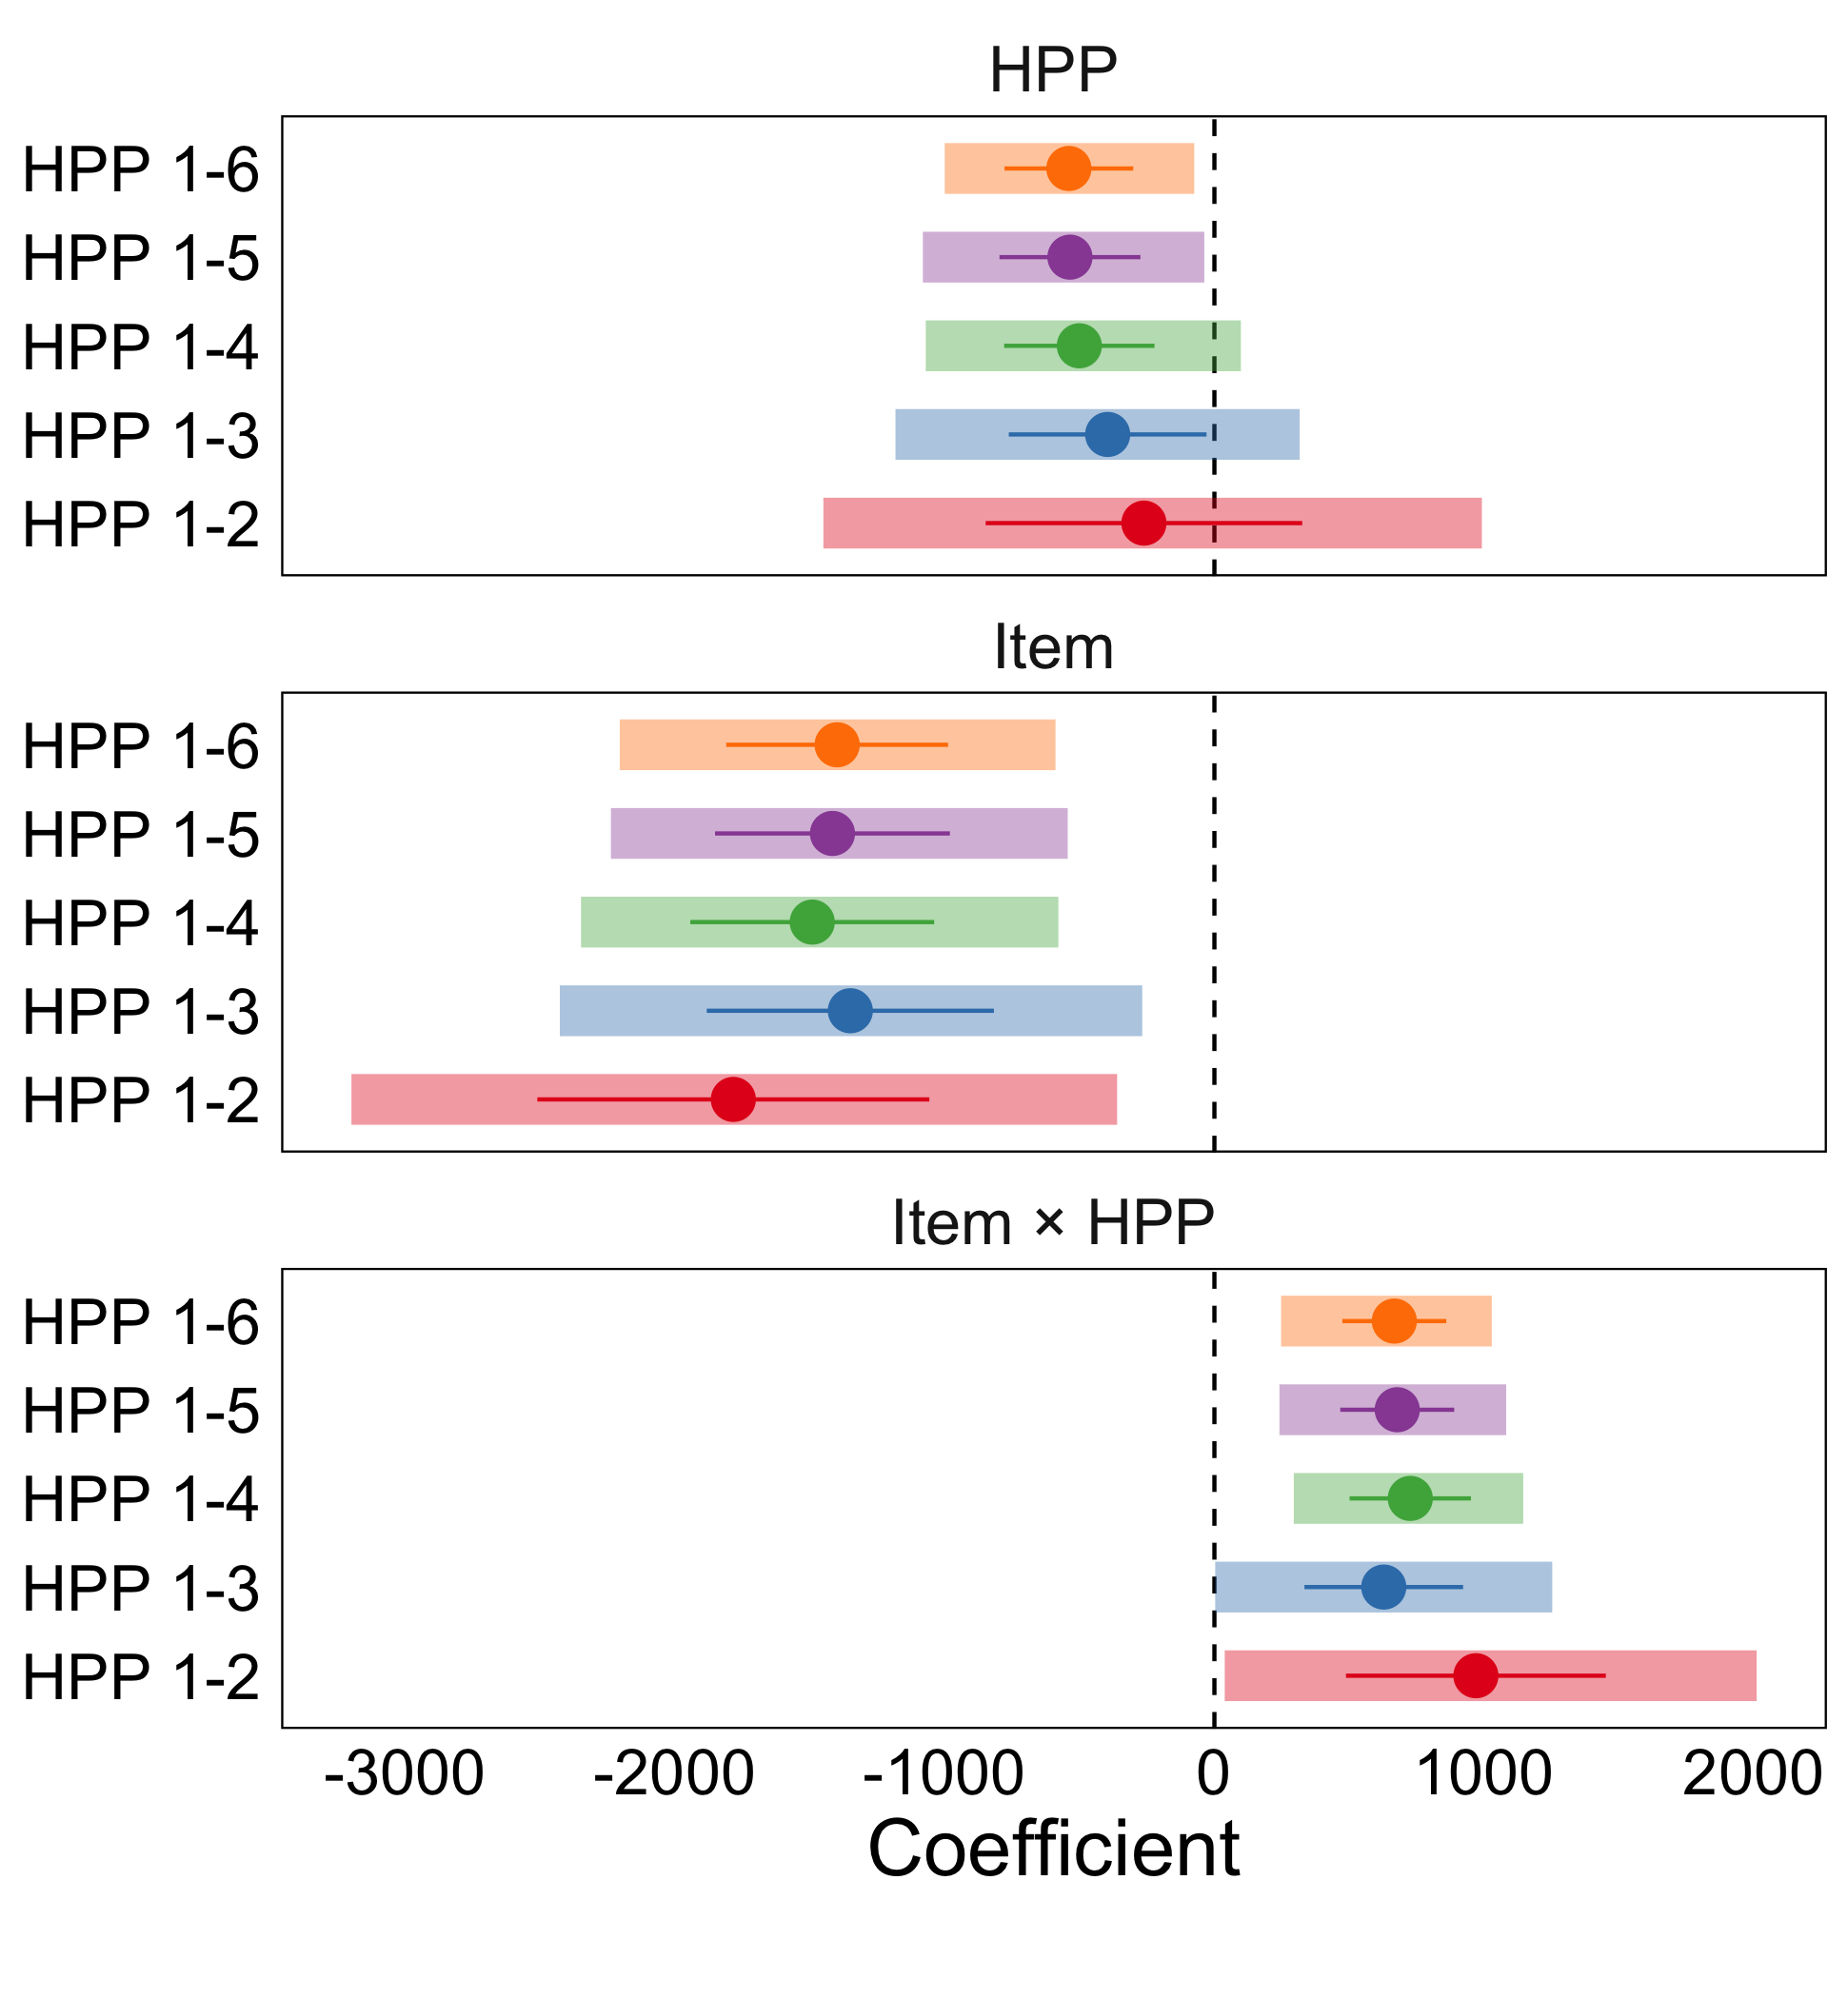
\includegraphics[width=\textwidth]{/Users/GonzaloGGC/projects/Flip/Figures/05_anova-merged} \caption{Graphical representation of the coefficients of the Test Item by HPP visits interaction term of the model fitted on the complete data-set (reported in the main manuscript), and of the models fitted on the reduced data-sets. Black dots represent the point estimate of the coefficient, black whiskers represent the standard error of the mean, and grey boxes represent the bootstrapped 95\% confidence interval around the point estimate.}\label{fig:unnamed-chunk-16}
\end{figure}

\hypertarget{session-info}{%
\section{Session info}\label{session-info}}

R version 3.5.1 (2018-07-02) Platform: x86\_64-apple-darwin15.6.0
(64-bit) Running under: macOS 10.15.2

Matrix products: default BLAS:
/Library/Frameworks/R.framework/Versions/3.5/Resources/lib/libRblas.0.dylib
LAPACK:
/Library/Frameworks/R.framework/Versions/3.5/Resources/lib/libRlapack.dylib

locale: {[}1{]}
en\_US.UTF-8/en\_US.UTF-8/en\_US.UTF-8/C/en\_US.UTF-8/en\_US.UTF-8

attached base packages: {[}1{]} stats graphics grDevices utils datasets
methods base

other attached packages: {[}1{]} purrr\_0.3.3 kableExtra\_1.1.0
ggplot2\_3.3.0\\
{[}4{]} here\_0.1-11 tibble\_2.99.99.9014 dplyr\_0.8.99.9000\\
{[}7{]} magrittr\_1.5 knitr\_1.27 papaja\_0.1.0.9942

loaded via a namespace (and not attached): {[}1{]} Rcpp\_1.0.4
pillar\_1.4.3.9000 compiler\_3.5.1\\
{[}4{]} highr\_0.8 lobstr\_1.1.1 base64enc\_0.1-3\\
{[}7{]} tools\_3.5.1 zeallot\_0.1.0 digest\_0.6.25\\
{[}10{]} viridisLite\_0.3.0 evaluate\_0.14 lifecycle\_0.1.0\\
{[}13{]} gtable\_0.3.0 pkgconfig\_2.0.3 rlang\_0.4.5.9000\\
{[}16{]} rstudioapi\_0.11 yaml\_2.2.1 xfun\_0.12\\
{[}19{]} xml2\_1.2.2 httr\_1.4.1 withr\_2.1.2\\
{[}22{]} stringr\_1.4.0.9000 hms\_0.5.3 vctrs\_0.2.99.9005\\
{[}25{]} webshot\_0.5.2 rprojroot\_1.3-2 grid\_3.5.1\\
{[}28{]} tidyselect\_1.0.0 glue\_1.3.1 R6\_2.4.1\\
{[}31{]} rmarkdown\_2.1.1 bookdown\_0.17 readr\_1.3.1\\
{[}34{]} backports\_1.1.5 scales\_1.1.0 htmltools\_0.4.0.9003 {[}37{]}
ellipsis\_0.3.0 rvest\_0.3.5 colorspace\_1.4-1\\
{[}40{]} stringi\_1.4.6 munsell\_0.5.0 crayon\_1.3.4

\hypertarget{references}{%
\subsection{References}\label{references}}

\begingroup
\setlength{\parindent}{-0.5in}
\setlength{\leftskip}{0.5in}

\hypertarget{refs}{}
\leavevmode\hypertarget{ref-barr2013}{}%
Barr, D. J., Levy, R., Scheepers, C., \& Tily, H. J. (2013). Random
effects structure for confirmatory hypothesis testing: Keep it maximal.
\emph{Journal of Memory and Language}, \emph{68}(3), 255--278.
\url{https://doi.org/10.1016/j.jml.2012.11.001}

\leavevmode\hypertarget{ref-bates2015a}{}%
Bates, D., Kliegl, R., Vasishth, S., \& Baayen, H. (2015a). Parsimonious
Mixed Models. \emph{arXiv:1506.04967 {[}Stat{]}}. Retrieved from
\url{http://arxiv.org/abs/1506.04967}

\leavevmode\hypertarget{ref-bates2015}{}%
Bates, D., Mächler, M., Bolker, B., \& Walker, S. (2015b). Fitting
linear mixed-effects models using lme4. \emph{Journal of Statistical
Software}, \emph{67}(1), 1--48.
\url{https://doi.org/10.18637/jss.v067.i01}

\leavevmode\hypertarget{ref-brauer2018}{}%
Brauer, M., \& Curtin, J. J. (2018). Linear mixed-effects models and the
analysis of nonindependent data: A unified framework to analyze
categorical and continuous independent variables that vary
within-subjects and/or within-items. \emph{Psychological Methods},
\emph{23}(3), 389--411. \url{https://doi.org/10.1037/met0000159}

\leavevmode\hypertarget{ref-fox2019}{}%
Fox, J., \& Weisberg, S. (2019). \emph{An R companion to applied
regression} (Third). Thousand Oaks CA: Sage. Retrieved from
\url{https://socialsciences.mcmaster.ca/jfox/Books/Companion/}

\leavevmode\hypertarget{ref-judd2012}{}%
Judd, C. M., Westfall, J., \& Kenny, D. A. (2012). Treating stimuli as a
random factor in social psychology: A new and comprehensive solution to
a pervasive but largely ignored problem. \emph{Journal of Personality
and Social Psychology}, \emph{103}(1), 54--69.
\url{https://doi.org/10.1037/a0028347}

\leavevmode\hypertarget{ref-rcoreteam2018}{}%
R Core Team. (2018). \emph{R: A language and environment for statistical
computing}. Vienna, Austria. Retrieved from
\url{https://www.R-project.org/}

\leavevmode\hypertarget{ref-saffran2008}{}%
Saffran, J., Hauser, M., Seibel, R., Kapfhamer, J., Tsao, F., \&
Cushman, F. (2008). Grammatical pattern learning by human infants and
cotton-top tamarin monkeys. \emph{Cognition}, \emph{107}(2), 479--500.
\url{https://doi.org/10.1016/j.cognition.2007.10.010}

\leavevmode\hypertarget{ref-saffran2003}{}%
Saffran, J. R., \& Wilson, D. P. (2003). From Syllables to Syntax:
Multilevel Statistical Learning by 12-Month-Old Infants. \emph{Infancy},
\emph{4}(2), 273--284. \url{https://doi.org/10.1207/S15327078IN0402_07}

\leavevmode\hypertarget{ref-santolin2019}{}%
Santolin, C., \& Saffran, J. R. (2019). Non-Linguistic Grammar Learning
by 12-Month-Old Infants: Evidence for Constraints on Learning.
\emph{Journal of Cognition and Development}, \emph{20}(3), 433--441.
\url{https://doi.org/10.1080/15248372.2019.1604525}

\leavevmode\hypertarget{ref-santolin2019a}{}%
Santolin, C., Saffran, J. R., \& Sebastian-Galles, N. (2019).
Non-linguistic artificial grammar learning in 12-month-old infants: A
cross-lab replication study. In. Potsdam, Germany.

\endgroup
\end{appendix}

\end{document}
